\documentclass[12pt,a4paper]{report}

\usepackage{dolgozat}

\usepackage{hyperref}

\usepackage{listings}
\usepackage{python}
\usepackage{java}

\usepackage{xcolor}
\usepackage{indicators}

\linespread{1.2}

\begin{document}

\pagestyle{empty} %a címlapon ne legyen semmi=empty, azaz nincs fejléc és lábléc

\begin{flushleft}
\textsc{\bfseries Miskolci Egyetem}\\
Gépészmérnöki és Informatikai Kar\\
Analízis Intézeti Tanszék
\end{flushleft}

%A fõiskola logoja
{\large
\begin{center}
\vglue 1truecm
\textbf{\huge\textsc{Szakdolgozat}}\\
\vglue 1truecm

\epsfig{file=cimlap/ME_logo.eps, width=4.8truecm, height=4truecm}\\
\textbf{\textsc{Miskolci Egyetem}}
\end{center}}

\vglue 1.5truecm %függõleges helykihagyás

%A szakdolgozat címe, akár több sorban is
{\LARGE
\begin{center}
\textbf{Fesztiválkereső webes alkalmazás}
\end{center}}

\vspace*{2.5truecm}
%A hallgató neve, évfolyam, szak(ok), a konzulens(ek) neve
{\large
\begin{center}
\begin{tabular}{c}
\textbf{Készítette:}\\
Bandur Martin\\
Gazdaságinformatikus BSc
\end{tabular}
\end{center}
\begin{center}
\begin{tabular}{c}
\textbf{Témavezetõ:}\\
Piller Imre, egyetemi tanársegéd
\end{tabular}
\end{center}}
\vfill
%Keltezés: Hely és év
{\large
\begin{center}
\textbf{\textsc{Miskolc, 2018}}
\end{center}}

\newpage


\pagestyle{empty}
\vspace*{1cm}  
\begin{center}
\large\textsc{\bfseries Eredetiségi Nyilatkozat}
\end{center}
\vspace*{2cm}  

Alulírott \textbf{Bandur Martin}; Neptun-kód: \texttt{NINH8N} a Miskolci Egyetem Gépészmérnöki és Informatikai Karának végzõs gazdasági informatikus szakos hallgatója ezennel büntetõjogi és fegyelmi felelõsségem tudatában nyilatkozom és aláírásommal igazolom, hogy
\textit{Fesztiválkereső webes alkalmazás}
címû szakdolgozatom/diplomatervem saját, önálló munkám; az abban hivatkozott szakirodalom
felhasználása a forráskezelés szabályai szerint történt.\\

Tudomásul veszem, hogy szakdolgozat esetén plágiumnak számít:
\begin{itemize}
\item szószerinti idézet közlése idézõjel és hivatkozás megjelölése nélkül;
\item tartalmi idézet hivatkozás megjelölése nélkül;
\item más publikált gondolatainak saját gondolatként való feltüntetése.
\end{itemize}

Alulírott kijelentem, hogy a plágium fogalmát megismertem, és tudomásul veszem, hogy
plágium esetén szakdolgozatom visszautasításra kerül.

\vspace*{3cm}

\noindent Miskolc, \hbox to 2cm{\dotfill} év \hbox to 2cm{\dotfill} hó \hbox to 2cm{\dotfill} nap

\vspace*{3cm}

\hspace*{8cm}\begin{tabular}{c}
\hbox to 6cm{\dotfill}\\
Hallgató
\end{tabular}


\cleardoublepage
\pagenumbering{gobble}
\tableofcontents
\cleardoublepage
\pagenumbering{arabic}

\newpage

\pagestyle{fancy}

\Chapter{Bevezetés}

% TODO: Itt kellene meggyőzni az olvasót, hogy milyen izgalmas, és fontos témáról van szó.
% A végén fixálandó

A rendszer segít eligazodni a fesztiválok világában, és az érdeklődőknek eldönteni, hogy melyik fesztiválon szeretne részt venni.

\Chapter{Fesztivál alkalmazások}

% TODO: Táblázatos formában a fő funkciókat összehasonlítani. (Sorokban a weboldalak, oszlopokban a funkciók, és pipálgatni, hogy melyiknél melyik van meg.)

Az elkészülő alkalmazás specifikációja előtt érdemes áttekinteni, hogy pontosan milyen szolgáltatások kapcsolódnak egy fesztiválhoz. Ez segít majd behatárolni az alkalmazás szükséges funkciót. Fontos továbbá ennek kapcsán megvizsgálni, hogy milyen hasonló alkalmazások érhetők már el, illetve azok milyen feladatokat és milyen formában látnak el.

\section{Fesztiválokhoz kapcsolódó szolgáltatások}

Először nézzük meg, hogy pontosan hogyan definiálhatnánk, hogy mi tekintünk fesztiválnak.

,,Fesztivál minden olyan – egy vagy több téma köré szerveződő, rendszeresen megrendezésre kerülő, egy vagy több helyszínen történő, meghirdetett programmal rendelkező kulturális, művészeti, gasztronómiai, sport vagy egyéb – eseménysorozat, melynek célja, hogy közönsége részére kiemelten színvonalas, értékközvetítő, minőségi, ismereteket is bővítő és egyben szórakoztató, szabadidős közösségi élményt nyújtson.'' (Magyar Fesztivál Szövetség, 2009) [21]

A hazai turizmus bevételeinek jelentős részét a program azon belül a fesztiválturizmus adja.

\begin{comment}{Az előző állítást valamilyen forrással, konkrét számadatokkal alá kellene támasztani.}
\end{comment}

A dolgozatomban a klasszikus értelembe vett zenei vagy zenei vonatkozású fesztiválokra fókuszálok.
A fesztiválokhoz nagyon változatos és sokrétű funkció csoportok tartoznak, melyeket több szempont alapján kategorizálhatunk. Az elkészülő szoftver funkcióinak behatárolásához, a követelményspecifikáció elkészítéséhez vegyük ezeket sorra.

\subsection{Közvetlenül kapcsolódó funkciók}

A fesztiválozáshoz, mint szolgáltatáshoz közvetlenül kapcsolódó funkciók az alábbiak.
\begin{itemize}
\item Fellépők, a legnagyobb vonzereje a szolgáltatásnak, ezeket kellő időben és helyen kell megismertetni a közönséggel. Ide értve nem csak a zenei produkciókat, de egyéb performance-t, és előadásokat, prevenciókat.
\item Élelmiszer és ital, a zenei fesztiválok jelentős része 3-10 napos periódusban gondolkodik. Alapvető szükségletet elégít ki, általában egy ilyen esemény alatt nagyobb összeget költenek erre a kategóriára, mint magára a belépőre, utazásra, szállásra.
\item Egyéb sport, kulturális, szellemi programok, vetélkedők. Technológiai bemutatók kipróbálási lehetőséggel.
\item VIP szolgáltatások, közönségtalálkozók.
\end{itemize}

\begin{comment}{Ezek itt jók, de át kellene fogalmazni, hogy tényleg funkcióra/szolgáltatásra vonatkozzanak.}
\end{comment}

\subsection{Közvetve kapcsolódó funkciók}

Közvetve kapcsolódó funkciók: Amelyeket nem érzékel, amikért nem fizetne önmagában, illetve nem kell tudnia a fesztiválozónak, de kényelmetlenül érezné magát, ha nem valósulnának meg. Ilyenek például az alábbiak.
\begin{itemize}
\item Takarítás, WC használat, esetenként a zuhanyzási és alvási lehetőség.
\item A színpadok, dekorációk, kerítések építése, karbantartása, lebontása.
\item A fellépők oda és haza juttatása zökkenőmentesen.
\item Készletgazdálkodás, promóciók, kérdőívek.
\item Média megjelenés.
\item Elektronikus, internetes hálózat, közvilágítás.
\item Biztonság, az időjárás viszontagságai ellen védelem, értékmegőrzés.
\item Rekreáció, egészségmegőrzés.
\item Fodrász, kozmetikus a feltűnő és kreatív megjelenés érdekében.
\item Véradásért cserében valamilyen ellenszolgáltatás.
\end{itemize}

\subsection{Az alkalmazás szempontjából kiemelt funkciók}

Melyek azok a szolgáltatások, amelyek érdekelni fogják a felhasználót, szeretne előretudni róla, és ezeket egy információs rendszerben meg lehet jeleníteni.
\begin{itemize}
\item Fellépők listája, mint már említettem ez az egyik legfőbb vonzerő.
\item Az extrém nem mindenhol kipróbálható sportolási, technológiai lehetőség.
\item Hasznos lehet a környékbeli étkezők elérhetősége, akár étlapja árakkal. Tudjuk, hogy a fesztiválok a magas áraikról és főleg a gyors kajáikról híresek. Érdemes lehet az olcsóbb, vagy a gasztronómia szerelmeseinek a környező elit éttermekről előre információt nyújtani.
\item Dohányboltok, illetve dohányzás. Magyarországon jelenleg a jogszabályi környezet befolyásolja a dohányáruk vásárlási helyét, erről nyújthat információt egy alkalmazás, és arról is, hogy lehetséges-e dohányozni a fesztiválterületen vagy sem.
\item Szállás, vannak olyan fesztiválok, amelyek sátorhelyet és/vagy faházat biztosítanak a közönségük számára. Emellett megjeleníthetőek a kollégiumok, apartmanok, szállodák.
\item Kutyabarátság, kutya bevihető-e a rendezvényre.
\item Gyerekbarátság, gyermekek bevihetőek-e, esetleg vannak-e számukra külön programok.
\item Jegyek, kell-e fizetnünk a fesztiválra belépésért vagy ingyenesen látogatható. Ha igen, akkor milyen jegytípusok érhetőek el.
\item Strandolási lehetőség. A zenei fesztiválok jelentős része nyáron van és vízközelben, hogy a közönségnek legyen lehetősége védekezni a meleg ellen.
\end{itemize}

\section{Konkurens alkalmazások}

Az interneten fellelhető már egypár elterjed Fesztivál/Esemény kereső alkalmazás, vannak hiányosságaik és tartalmaznak frappáns ötleteket is. A következő szakaszok ezeket tekintik át.

\subsection{Fesztiválkalauz.hu}

1. http://www.fesztivalkalauz.hu : Az első dolog amivel a felhasználó találkozik az a felhasználói felület, amelynek körülbelül a felét használta ki a fejlesztő. Jelenleg egy 14"-os kijelzőn nézve ez zavaróan kicsi. Feltehetőleg ez azért is van így, mert nagyjából 10 éves fejlesztés, és akkor még nem volt ekkora kijelző választék - sem méret, sem eszköz tekintetében - amelyeken weboldalakat jelenítettünk meg, így elég volt egy statikus méretre és betűtípusra beállítani a weboldalt. Jelenleg divatosak a reszponzív weboldalak, amelyek igyekeznek kiküszöbölni ezt a problémát.
[1] A reszponzív weboldal (RWD) egy olyan megközelítéssel tervezett weboldal, amelynek a célja az, hogy optimális megjelenést biztosítson - könnyű olvashatóság, egyszerű navigáció a lehető legkevesebb átméretezéssel és görgetéssel - a legkülönfélébb eszközökön (az asztali számítógép monitorjától egészen a mobiltelefonokig).
A viszonylag fejlett fesztiválkereső nekem tetszik, sok mindenre rálehet keresni, könnyen és átláthatóan.
Lehet település, kerület, illetve megye szerint is keresni. Típus és dátum szerinti keresés is támogatott. Sőt módunkban áll a következőhavi eseményeket is lekérdezni egy kattintással, erről ha szeretnénk, hírlevelet is kérhetünk. A szabad szavas kereső, annyira azért mégsem szabad, mert csak a címben keres a leírásban sajnos nem.

\subsection{Utazzithon.hu}

2. https://www.utazzitthon.hu/program : Az oldal mint a szlogenje is mondja: "Belföldi szállás, program és látnivaló 1 helyen", szállásokat és programokat közvetít az érdeklődőknek. A felület már reszponzív tervezés eredménye, ennek köszönhetően átlátható és könnyen használható akár mobileszközről is. A keresés nagyon világos, kereshetünk régió, tájegység, város szerint és program, látnivaló típusok alapján. Az adatbázisuk programok tekintetében elég gazdag, amikor megtekintettem közel 8000 programot ajánlottak. Itt jegyet is vásárolhatunk az egyes programokra.

\subsection{Fesztival.eu}

3. http://www.fesztival.eu/: A weboldal régi dizájnnal készült. A keresője nagyjából hasonló funkciókat tükrözött, mint az eddigiekben megjelenő keresési lehetőségek. Sajnos az adatbázisában csak egy fesztivál volt megtalálható, amikor ott jártam, így tesztelni nem volt módom.

\subsection{Fesztiválnaptár.hu}

4. http://www.fesztivalnaptar.hu : Az iranymagyarorszag.hu által működtetett weboldal. Feltehetően az utazzitthon.hu-hoz hasonlóan a szállások közvetítése a főprofilja, és ezek mellé jönnek be a fesztiválok, koncertek mint kiegészítőszolgáltatások. Szabad szavas kereséssel és kronológiai sorrend szerinti érhetőek el a programok. A szabad szavas kereső viszont keres a leírásban is, ami sokat könnyít a felhasználó számára. A felület nem reszponzív és régebbi stílusú. Nem nagy meglepetés, hogy 100-nál kevesebb esemény programját találjuk meg. Itt jelenik meg egyedül a nemzetköziesítés, a magyaron kívül angolul és németül is elérhetőek a programok, habár a programokhoz tartozó leírások csak magyarul érhetőek el.

\subsection{Programturizmus.hu}

5. https://www.programturizmus.hu/ : Az utolsó keresést támogató rendszerhez érkeztünk amit találtam, és szerintem a legletisztultabb felülettel és szolgáltatásokkal. Természetesen modern weboldal lévén, platformtól és kijelző mérettől függetlenül szépen megjelenik bármilyen eszközön. Az oldal nem csak fesztiválokra, hanem szinte minden olyan lehetőséget hivatott bemutatni, ami kimozdítja a fotelból a felületen böngésző felhasználót, ez a hozzáállás a szlogenben is tükröződik - "Ne maradj otthon!". Találunk itt a vásárok, látnivalók, és gasztronómián belül, Kolbásztöltő versenytől, a Kutyakiállításon át a Régiségvásárig mindent. Persze megjelennek a már klasszikusnak mondható szállások is. A keresés a már az előzőekben megszokott lehetőségek szerint lehetséges. Viszont az "Események" mellett megjelenik három új lehetőség is, az egyik az "Ajánlat" menü, a másik az "Érdekesség", ezek valami alapján kitüntetett események, viszont az utolsó talán a legérdekesebb. Ez pedig a koordináták alapján megmutatja, hogy hol is lesznek helyileg az események egy google térképen. A jegyet itt is vásárolhatunk. Ha egy fesztivált részletesebben megnézünk, meglepőmódon a jegyen, a címen és szálláson kívül még a környékbeli étkezési lehetőségeket is tanácsolja számunkra a weboldal.

\subsection{Élményem.hu}

5+1. http://elmenyem.hu : Az oldal nem rendelkezik fesztiválkereső résszel, ez inkább egy blog. De rengeteg aktualitással, hírekkel szolgál a jövőben megrendezendő eseményekkel kapcsolatban. 

\section{További lehetséges szolgáltatások}

Az itt felsorolt weboldalak természetesen a jövőben változásokon eshetnek át. Ezek a szakdolgozat írás közbeni állapotokat tükröznek.

Extra lehetőségek, amelyekkel nem éltek az itt feltüntetett weboldalak:

SZÉP-kártya, és egyéb fizetési lehetőségek feltüntetése.

Gyerek illetve kutyabarát-e a rendezvény. Könnyen megvalósítható, mégis látványos lehetőségeket rejt magában, hiszen egy cumi, vagy egy mancs elhelyezése az esemény mellett vagy alatt, adatbázis szinten pedig csak egy boolean változó bevezetése.

Dohányzásra, alkoholfogyasztásra, korhatárra is lehetne bevezetni hasonló kis ikonokat, ezeket is egyszerű paraméterként fel lehetne szerelni.
Értékmegőrzésre, telefon töltésre van-e lehetőség. 
Ingyenes-e a rendezvény: Ez is könnyen felkeltheti az érdeklődők figyelmét. Itt is alkalmazható lenne a már jól bevált ikonos megoldás.
A nemzetköziesítés is szempont lehet, habár ezek az oldalak elsősorban hazai piacra készültek, amelyek fesztiválok nemzetközi vendégeket várnak, azoknak a marketingprogramja is külföldre pozíciónál, és saját weboldallal is rendelkeznek. Ideértve az árak több valutában való megjelenítését is a leírások szövege mellett.

Közlekedés: Érdemes lehet feltüntetni, magát a fesztivál koordinátáit, mint ezt a programturizmus.hu weboldalon láthattuk, emellett érdemes lehet parkolási lehetőségekről térképen előre informálni az odaérkezőket, egy nagyobb eseményre akár több ezer személyautóval is érkezhetnek. A buszpályaudvarról és vasútállomásról a célhoz eljutást segítő helyi járatok menetrendjét is lehetne mellékelni. Az eseménnyel szerződött taxivállalatok telefonszámait felsorolni. A gyalogos eljutást térkép segítségével megmutatni.

Szállás: Mint láthattuk, majdnem mindegyik weboldal ajánlott szállást hotelekben. De a fesztiválok klasszikus közönsége, az nem szállodákban alszik. Általában sátorban, faházakban, kollégiumokban, vagy épp ahol eléri az álom. Érdemes lenne jelezni a felhasználó felé, hogy lehet-e sátrazni, és ha igen, van-e ennek extra költsége. A kollégiumokat, faházakat is lehetne ilyen módon jelezni.

Időjárás: Ez sajnos nem jósolható hónapokkal előre, de pár héttel a fesztivál kezdete előtt ez is felkerülhetne. Hisz mint tudjuk, ezen események javarészt fedetlen vagy részben fedett helyeken zajlanak.
Visszacsatolás: A legtöbb ilyen eseményt többször megrendezik, vannak olyanok amik már 20-30 éves hagyományra tekintenek vissza. Így az értékelések, mind a szervezők, mind a szolgáltatást igénybe vevők számára hasznos információt nyújtanak.

Étkezés: Amire csak a programturizmus.hu gondolt, és alapvetően egy jó kis kiegészítő szolgáltatás, hisz fiziológiai szükségletet elégít ki.

\Chapter{Az alkalmazás specifikációja}

% TODO: képernyőképekhez vázlatos jellegű ábrák.
% TODO: Be kellene mutatni néhány használati esetet is.

Az alkalmazás célja, hogy a kisebb fesztiválok versenyhelyzetét javítsa a nagyobbakkal szemben és ezeket eljuttassa a célközönséghez. A felhasználó által ismeretlen zenészeket megismertesse velük és közelebb hozza hozzájuk.

A fejezet összefoglalja, hogy melyek azok a funkciók, amelyekre szüksége lehet a felhasználóknak, így azt az alkalmazásban célszerűnek tűnik megvalósítani.

\section{Kereső funkciók}

Fesztiválkereső alkalmazásról lévén szó, így a webalkalmazásunk legfőbb funkciója a fesztiválozni vágyó tömeg számára az értékrendjük szerint releváns fesztiválok megtalálása, és ezekről a legkülönfélébb információk eljuttatása a célközönségük számára. A fesztiválok megkeresése a lehető legtöbb kritérium alapján megvalósulhasson. Továbbá szeretnénk ajánlani szállásokat és egyéb szolgáltatásokat amikkel élhetnek a fesztivál területén és közvetlen közelében.

\subsection{Keresési kritériumok}

Egy fesztivált talán a neve alapján a legkönnyebb azonosítani, ez azok számára könnyíti meg a dolgot, akik már tudják, mit keresnek csak extra információkat szeretnének gyűjteni a fesztiválról vagy a környezetéről (például szálláshelyek, vagy étkezési lehetőségek).

A második keresési szempont a település szerint, illetve településtől való távolság alapján. Gyakran fontos szempont lehet, hogy ne kelljen sokat utazni a kikapcsolódásért. Előfordul, hogy csak egy-egy nap programja érdekli a felhasználót. Ilyen esetben jó eséllyel nem fog szállást keresni, hanem még aznap haza szeretne utazni. Ezt a keresés természetesen kibővül, egy adott településtől való távolság szerinti keresésre, vagy akár regionálisra is bővülhet, például Balatonhoz közeli fesztiválok.

A következő kritérium amire szűrhetünk az a dátum. Mindenkinek az életében vannak olyan időpontok, időszakok amelyek terheltebbek, illetve kevésbé terheltek. Sokan dolgoznak külföldön és nem minden hétvégén tudják itthon tölteni. Időintervallum szerinti szűrés azon fesztiválok megtalálásában segít, amelyek akkor kerülnek megrendezésre, amikor ráérünk.

Fellépő alapú keresés, a felhasználók túlnyomó része az alapján is szelektálja a fesztiválokat, hogy ott lesznek-e a kedvenc fellépői vagy sem. Így természetesen a fellépő alapú szelekciót is meg kell valósítani. Ezt a részt úgy képzelem el, hogy a fellépőre kereshetünk rá és neki láthatjuk a fesztiválnaptárját, tehát, hogy hol és mikor lép fel. Külön menüként valósul meg.

Stílus alapján is megtalálhatjuk a fesztiváljainkat. Egyesek számára például az is fontos, hogy milyen stílusú a fesztivál. Itt a stílus alatt elég sok mindent érthetünk, például vannak tematikus fesztiválok amelyek, valamilyen étel vagy ital köré szerveződő fesztiválok, vannak amik a kultúra vagy művészettel kapcsolatosak, illetve a zenei fesztiválok. A stíluson belül további stílusokra, jellemzőkre oszlik egy fesztivál jellege:  milyen stílusú zenét játszanak a fesztiválon. Jellemzők alatt mit érthetünk? Állatbarátok számára fontos lehet, hogy bevihetik-e  a kis kedvenceket. A dohányzók számára a dohányzás szabadsága, a távolról érkezők számára  a sátrazás lehetősége. Ezekre a jellemzőkre utaló kulcsszavakat kell bevezetni, amelyek segítségével szintén könnyebben eligazodhat a fesztiválozni vágyó felhasználó. Ezekre a kulcsszavakra kattintva leszűrjük számára a megadott jellemzőkkel rendelkezőket.

Árkategória szerint is érdemes lehet szűrni. Elképzelhető, hogy valaki számára csak a teljesen ingyenes fesztiválok férnek bele a költségvetésébe, míg lehetnek olyan felhasználók is akik inkább a drágább fesztiválokat kedvelik mert ott feltehetőleg magasabb minőségűek a szolgáltatások, akár a közönség találkozhat személyesen a fellépővel vagy a jobb higiéniai és biztonsági feltételek miatt is választhatja, mindenki döntse el maga. Ez elképzelhető, hogy nem kerül implementálásra, mert a jegyekhez külön szakértelem kell. Miért mondom ezt? Egyszerűbb esetben van 2 verzió vagy van jegy vagy nincs. Ezt egy metaadat segítségével egyszerűen kiszűrhetjük, a metaadatunk lehet az előző pontban említett fesztiváljellemző. Bevezetve az ingyenes fesztiválokra egy, \#free, \#nincsBelépő vagy \#ingyenes kulcsszavakat. Viszont, ha van jegy, csak akkor van egyszerű dolgunk, ha csak egy fajta jegyünk van. Sajnos ez jellemzően nem így van. Általánosságban elmondható, hogy van a fesztiválon eltöltött napok szerint létező, szinte összes kombináció. Szállással kérjük vagy anélkül, és ha szállással akkor milyen szállással? A legtöbb fesztiválnak vannak szerződött partnerei, szállodák vagy kollégiumok illetve helyben is megtalálhatóak a sátorhelyek, faházak, lakókocsik, és tematikától függően még kitudja milyen alvási és pihenési lehetőségekkel nem futhatunk össze. Gyakran időintervallumhoz kötődnek a jegyárak, minél korábban veszünk meg egy jegyet annál olcsóbb. Vannak VIP jegyek, melyek az extra szolgáltatást igénylők számára lehet érdekes. És még lehetnek egyéb horizontok is, amik színesíthetik ezt a palettát, mostanában divat lett a buszok szervezése, főleg a  külföldi fesztiválokra, itt ismét megjelent egy plusz jegytípus. Lehetnek egyéb kedvezmények, és kuponok is. És ezeknek a kombinációja. Lássuk be, hogy ezeket a dolgokat és a változásaikat csak akkor lehetne jól kezelni, ha valamilyen API-n megkapnánk őket. De ezt az is gátolja, hogy ahány jegy annyi forgalmazó, mindenkinek a rendszerére nem lehet felkészíteni a mi rendszerünket, így maradunk annál a megoldásnál, hogy egy linket adunk, ahol mindenki kedvére válogathat a jegyek közül.

\subsection{Fellépők listázása és keresése}

\ref{fig:artist_search}. ábra alapján elmondhatjuk, hogy a felső blokkban található a kereső rész, minden leütött karakter után keres, név és/vagy stílus alapján. Ha üres a mező akkor az összes fellépőt listázzuk. Az alsó blokkban szereplő két kártya a listázás eredményét mutatja, természetesen nem feltétlen kettő lesz. Hanem annyi, amennyi megfelel a keresési kritériumoknak. A kártyán szerepel a fellépő neve, egy kép róla, egy rövid leírás, a stílusainak listája, és egy részletek gomb. A részletek gombra kattintva a Fellépő részletei(\ref{fig:artist_details}. ábra) elérhetővé válnak.

\begin{figure}
\centering
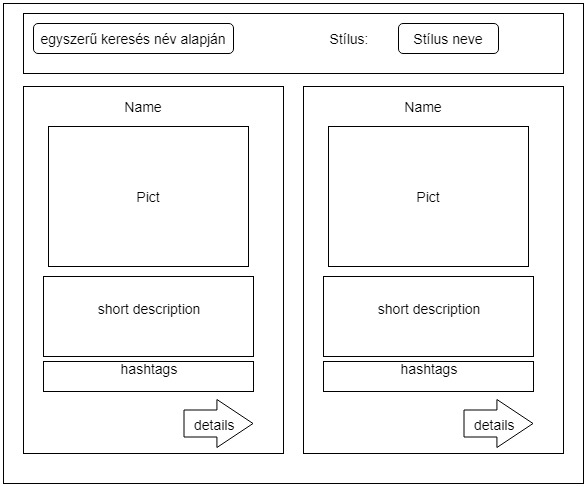
\includegraphics[scale=0.5]{kepek/artist_search.jpg}
\caption{Fellépők keresése}
\label{fig:artist_search}
\end{figure}

\subsection{Fellépő részletei}

Alapvetően ugyanazok találhatóak meg rajta, mint a \ref{fig:artist_search}. ábrán fellelhető kártyákon, ez mindösszesen a fellépő koncertjeivel bővül.

\begin{figure}
\centering
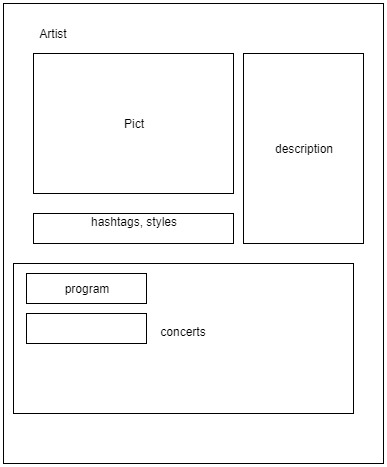
\includegraphics[scale=0.5]{kepek/artist_details.jpg}
\caption{Fellépő részleteiben}
\label{fig:artist_details}
\end{figure}

\subsection{Fesztiválok listázása és keresése}

A Fesztiválok listázása (\ref{fig:fest_search}. ábra) nem sokban tér el a Fellépők listázásától. A keresés blokk a fesztiválok esetében sokkal bővebb. Ezt főképen annak köszönheti, hogy több numerikus adatot tudunk hozzárendelni, így intervallumban is lehet keresni.
A felső blokk egy szimpla név alapú keresés lesz. 

A második blokkban
\begin{itemize}
\item stílus alapján,
\item ingyenesség alapján,
\item egy településen és a településtől megadott távolságon belül megrendezett, 
\item két dátum közötti időintervallumban megrendezésre kerülő
\end{itemize}
és ezek kombinációinak alapján tudjuk kilistázni az eseményeket.

A kártyán szerepel a fesztivál neve, egy molinó vagy egyéb kép róla, egy rövid leírás, a stílusainak listája, a település ahol megrendezésre kerül, a  fesztivál kezdetét és végét jelző dátum és egy részletek gomb. A részletek gombra kattintva átirányít a program minket a kiválasztott esemény részleteihez.

\begin{figure}
\centering
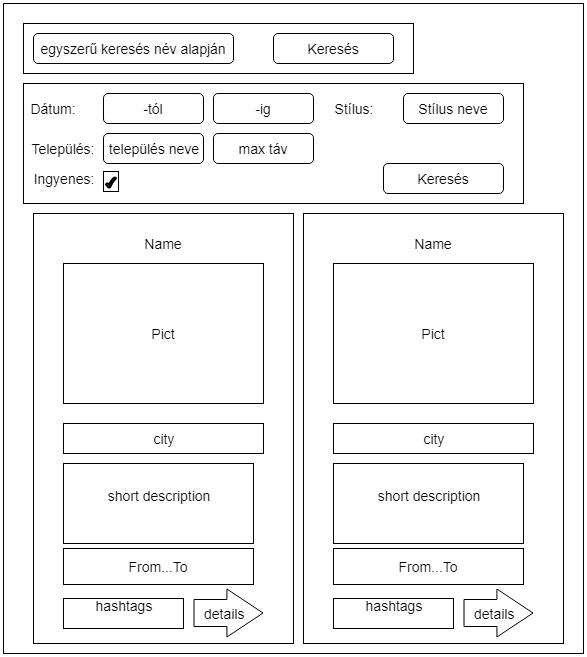
\includegraphics[scale=0.5]{kepek/fest_search.jpg}
\caption{Fesztiválok keresése}
\label{fig:fest_search}
\end{figure}

\subsection{Fellépő részletes adatai}

A fesztivál részletei oldalon elérjük azokat az adatokat mint a listázásnál a kártyán, illetve találunk itt egy linket a jegyekhez. A fesztiválon megrendezésre kerülő koncertek listáját. Illetve ajánlunk a felhasználó számára néhány szállást a fesztivál közelében (\ref{fig:artist_details}. ábra).

\begin{figure}
\centering
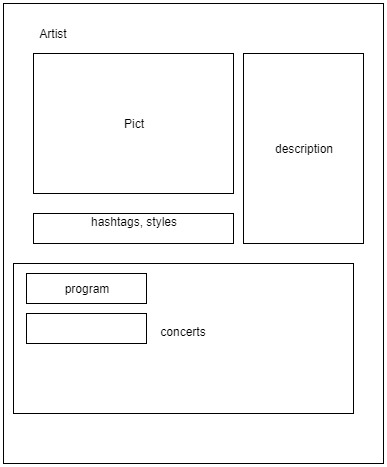
\includegraphics[scale=0.5]{kepek/artist_details.jpg}
\caption{Fesztivál részletei}
\label{fig:artist_details}
\end{figure}

\section{Kiegészítő funkciók}

A keresés mellett például az alábbi funkciók megvalósítása tünt még célszerűnek.
\begin{itemize}
\item A fesztivál megtekintésekor, mutassuk meg a fesztivál közelében levő szállási lehetőségeket, éttermeket, egyéb rekreáció és a fesztiválozáshoz kapcsolható szolgáltatásokat. Én csak a szállásokkal tervezem feltölteni az adatbázisom, de természetesen ugyanúgy lehetne biciklikölcsönzőt vagy strandot is mutatni a fesztiválterület közelében.
\item A teljes fesztivál programot elérhetővé kell tenni a fesztivál oldalán. És ha valamelyik koncert fellépőjére kattintunk, akkor tudjuk elérni a hozzá tartozó profilt. Ahol elolvashatjuk a fellépőről szóló leírást, és akár a weboldalát vagy a YouTube csatornáját is elérhetjük, ahol belehallgathatunk a népszerű slágereikbe.
\item Az ezt megelőzőt fordítva is szeretnénk elérni. Tehát, ha kiválasztunk egy fellépőt a listából, akkor lássuk egyben a fesztivál naptárját, hol fog és mikor fellépni. És természetesen itt is el kell tudnia érni azokat a fesztiválok oldalát amelyek ezek közül érdeklik.
\end{itemize}

\section{Felhasználói adatok kezelése}

A weboldalakon jellemzően megjelenik a felhasználói fiók kezelése mint funkció. Így ennek a mi rendszerünkben is helye lesz.
Több funkciót kell megvalósítanunk. Melyek is ezek?
\begin{itemize}
\item Belépés: A rendszerbe már regisztrált felhasználó a felhasználónevének és jelszavának megadásával belép a rendszerbe és eléri annak funkcióit. Természetesen ehhez a felhasználónév és jelszó párost helyesen kell megadnia, különben a rendszerünk elutasítja a bejelentkezési szándékot.
\item Kilépés: A felhasználó kilép a rendszerből, innentől már nem érheti el azon funkciókat, amelyek csak az autentikált felhasználó privilégiumai.
\item Regisztráció: A felhasználó egy űrlap kitöltésével regisztrálhat a rendszerbe, ha minden kötelező adatot kitöltött és azok megfelelnek a formai követelményeknek.
\end{itemize}

\subsection{Jogosultsági körök}

\begin{itemize}
\item ADMIN: Az admin - más néven adminisztrátor - az a jogosultsági kör aki felviheti a rendszerbe a felületen keresztül a fesztiválokat, szállásokat, és a fellépőket. Mindezeket törölheti és módosíthatja is az adatbázisban, de természetesen a felhasználói felületen keresztül is. ADMIN jogosultságot legtöbb esetben nagyon kevés felhasználó kaphat. Az előzetes terveim szerint egyenlőre aki hozzáférést kap a rendszerhez az ADMIN lesz. De egyenlőre csak korlátozott számú ilyen személy lesz.
\item USER: Az a felhasználó aki be van jelentkezve a rendszerbe, de módosítani nem tudja azt, esetleg módosítási javaslatokat tehet. Lehetősége van feliratkozni egyes zenekarokra, illetve fesztiválokra és levelet kaphat róla, ha valami módosul. Ez a felhasználó nem biztos, hogy megvalósul a fejlesztés ezen fázisában, majd az időkorláttól is függ. Vagy pedig minden user egyben admin is lesz.
\item Be nem jelentkezett felhasználó: Mindent megtekinthet, de módosítani nem tudja a rendszerben lévő adatokat, ahogy új adatot sem tud felvinni, és törölni sem tudja azokat.
\end{itemize}

\subsection{Regisztráció}

A regisztrációhoz meg kell adni a \ref{fig:registration}. ábrán megadott paramétereket. Sorrendben a következőket: felhasználónév, teljes név, email, a jelszót kétszer, hogy megegyezik-e mindkettő. Egy kép feltöltésére is van lehetőség, ez lesz a profilkép. A küldés gombra kattintva lementődik a profil, ha a felhasználónév még nem létezik.

\begin{figure}
\centering
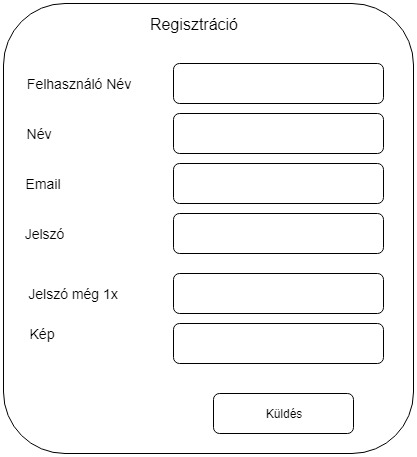
\includegraphics[scale=0.5]{kepek/registration.jpg}
\caption{Felhasználó regisztrációs űrlap}
\label{fig:registration}
\end{figure}

\subsection{Bejelentkezés}

A bejelentkezéshez csak egy egyszerű felhasználónevet és jelszót bekérő űrlapot (\ref{fig:login}. ábra) fogunk használni, melyet a login gombra kattintva küldhetünk el ellenőrzésre. Ha létezik a felhasználónév és a jelszót sem rontottuk el, akkor beengedi a felhasználót, egyébként egy hibaüzenetet küldünk neki, hogy valamit elrontott.

\begin{figure}
\centering
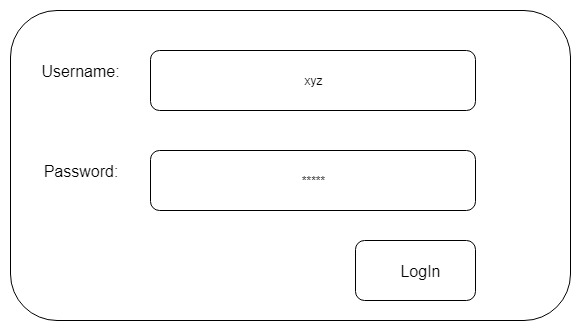
\includegraphics[scale=0.5]{kepek/login.jpg}
\caption{A bejelentkezési képernyő}
\label{fig:login}
\end{figure}

\section{Felvitel és módosítás}

\subsection{Szállás felvitele}

A szállások felviteléhez, meg kell adni a legfontosabb információkat a szállással kapcsolatban. Itt meg kell adni a szállás nevét, árát, a befogadható személyek számát és egy rövid leírást is adhatunk meg hozzá. Ezenkívül az kontakt adatokat is meg lehet adni, melyek emailcím, telefonszám, és a szállás weboldala. A szállás címével kapcsolatos adatokat is érdemes felvinni. Ha mindent megfelelően kitöltöttünk, akkor a    rögzítés gombra kattintva rögzíthetjük a szállást.

\subsection{Koncert felvitele}

A koncertek felviteléhez meg kell adni a fesztivált és a fellépőt, illetve hogy mikor kezdődik a koncert. minden adat kiválasztása kötelező.

\subsection{Fellépő felvitele}

Meg kell adni a fellépő nevét és a leírását illetve a hozzátartozó stílusokat, ha szeretnénk felvinni egy fellépőt. A stílusok kivételével a többi megadása kötelező, ha rögzíteni szeretnénk az adatbázisunkban.

\subsection{Esemény felvitele}

Egy esemény felviteléhez szükségünk lesz a nevére, a címére és a koordinátáira és a stílusaira egy részletes leírásra és végül két dátumra, arról hogy mikor kezdődik és mikor ér véget az esemény.

\subsection{Módosítás}

Módosításhoz is ugyanazok az űrlapokra lesz szükség mint amit az új felviteléhez használtunk, csak ott már be kell tölteni az aktuális adatokat.

\begin{comment}{ Ezekhez készülhet majd még ábra ha időm engedi vagy igény mutatkozik rá}
\end{comment}

\Chapter{Tervezés}

% TODO: Adatbázis sémájának a definíciója.

% TODO: Az architektúra bemutatása, hogy hol milyen technológia került felhasználásra. (A szokásos szerver-kliens kialakítás néhány egyedi dologgal.)

% TODO: Az alkalmazás felépítéséről UML ábrák. Minél részletesebben bemutatva, hogy minek kellene majd elkészülnie.

\Chapter{Implementáció}

A fejezetben bemutatok néhány izgalmasabb esetet, amelyek megvalósítása komplikáltabb volt, szakmai szempontból érdekesebb kihívást jelentettek.

\Section{Fesztivál keresés}

A fesztiválok megkereséséhez használtam a legkomplexebb folyamatot. A felület először azt vizsgálja meg, hogy melyik keresési paramétereket adta meg a felhasználó, és csak azokat a paramétereket küldi el a szerveroldalra, amelyek rendelkezésre állnak. Az $x$ és $y$ koordinátát egy Google maps API-n keresztül szerzem meg. Amikor beírja a felhasználó a kívánt települést, a rendszer pedig már a településhez tartozó koordinátákkal dolgozik tovább. Ha nem ír be semmit, akkor ezek az értékek üresek maradnak és a helytől való távolságot sem érdemes elküldeni. Amint látható a \texttt{HttpParams} objektumnak csak szöveg típusú változókat lehet átadni, így számértékkel kellett konvertálni. A dolog érdekessége, hogy a Spring oldalon ki lehet venni más típusként is.

A lekérdezésből visszaérkezett adathalmazt leképezzük a modellnek megfelelő formára és a modellekből készült tömbbel tér vissza a metódus a megjelenítési réteghez.

A metódus egyik paraméterét sem kötelező átadni neki, hisz ez egy lekérdezés, jöhet kevesebb információval is kérés. Ha érkezik dátum érték azt \texttt{Date} formátumra kell konvertálnunk és csak ezután hívhatjuk meg a a \texttt{FestivalService} \texttt{festsByQuery} metódusát.

A \texttt{festsByQuery} metódust implementáltam A \texttt{FestivalServiceImpl} osztályban. A függvény paraméter szignatúrája a következő:
\begin{java}
festsByQuery(
    String style,
    boolean isFree,
    Date begin, Date end,
    Double posX, Double posY,
    Double maxFromPos)
\end{java}
a visszatérési értéke egy \texttt{FestivalDTO} lista. A rendszert minden egyes lehetséges kombinációra fel kell készíteni. Természetesen lesznek olyan lekérdezések, amelyeket többször is meghívhatóak más paraméterrel. Ez abból ered, hogy az ingyenességet nem logikai változóban tárolom, hanem stílusparaméterként.

Amennyiben nem kapunk stílust akkor az alábbi ágba fut a programunk.
\begin{java}
if (!isFree) {
    festivals =
        datesWithoutStyle(begin, end, posX, posY, 
maxFromPos);
} else {
    festivals = datesWithStyle("free", begin, end, posX, posY,
    maxFromPos);
}
\end{java}

Abban az esetben, ha a felhasználó nem pipálta be, hogy ingyenes legyen a kiválasztott fesztivál, akkor lekérdezzük az adatbázisból a megadott dátumok szerinti eredményt.
Természetesen itt is előfordulhat, hogy nem adott meg dátumokat. Mind a négy lehetséges esetben már belenyúlunk az adatbázisba. Ha sem a kezdő, sem a végdátuma nincs megadva az intervallumnak amelybe keresünk, akkor mindent visszaadunk ami jelen pillanatban még nem fejeződött be.

\begin{java}
festivalRepository.findByEndDateAfterOrderByBeginDate(
    new Date(begin.getTime() - 1)
);
\end{java}

A fenti kódot használhatjuk, ha ismerjük az intervallum kezdetét, de a végét nem. Az előző esetben is ezt a kódot kell használni csak a pillanatnyi dátummal meghívva.
A kód a \texttt{CrudRepository} kiterjesztésével létrehozott \texttt{FestivalRepository} interfészt hívja meg amelyben ha bizonyos név konvenciókat betartunk, akkor automatikusan legenerálja a \texttt{Query}-t (lekérdezést) számunkra. De mint látható ez meglehetősen hosszú metódus neveket szül. A függvény az alábbi paraméterrel azokat adja vissza, amelyiket fesztiválokat a megadott pillanattól kezdve még érdemes meglátogatni. A dátumból az 1 érték kivonására azért van szükség, mert csak a $<$ összehasonlítás áll rendelkezésre, így a $\le$ megvalósításához a dátumot kell ennem megfelelően korrigálni.

\begin{java}
findByEndDateAfterAndBeginDateBeforeOrderByBeginDate(
    new Date(), new Date(end.getTime() + 1)
);
\end{java}

Amennyiben, ha csak azt adja meg a felhasználónk, hogy melyik időpontig alkalmas neki, akkor a \texttt{FestivalRepository} fenti függvényét érdemes meghívni a megadott paraméterekkel.
Szintén ez a függvény lesz jó nekünk arra, ha mindkettő dátum benne van a kérésben. Az első paramétert le kell cserélnünk \texttt{new Date(begin.getTime() - 1)}-re, hiszen itt megvan adva a \texttt{begin} érték is.

Ezek után a visszakapott értékekkel meg kell hívni a \texttt{workWithPositions(festivals, posX, posY, maxFromPos)} függvényt a megadott szignatúrával. Ez a függvény a \textit{Haversine} formula segítségével megvizsgálja a megadott paraméterek alapján az átadott fesztiválokat. Ha nem kaptunk pozíciót akkor vissza adunk mindent, ha csak pozíciót kaptunk, akkor az 5 km-en belülieket adjuk vissza, ha kapunk távolságot és pozíciót, akkor a pozíciótól megadott távolságon belüli fesztiválokat adja vissza.

Elképzelhető az is, hogy kiválasztotta a felhasználó, hogy ingyenes fesztiválok érdeklik, vagy esetleg stílust adott meg. Előfordulhat az is, hogy mindkettőt megadta a felhasználó. Mindhárom esetben a fesztivál keresés részben megadott kód \textit{else} ágában lefutó \texttt{datesWithStyle} függvényre lesz szükségünk, ami nagyon hasonlóan fog működni, mint a \texttt{datesWithoutStyle} csak a lekérdezés összes ágában össze kell kapcsolni a \texttt{FestivalStyle} táblával és onnan lekérdezni azokat amelyiknek a \texttt{style} mezője tartalmazza az átadott értéket, a további műveletek már nem változnak ugyan azokon a függvényhívásokon kell átesnie a visszakapott listának. A teljesség igénye nélkül nézzünk meg egy ilyen lekérdezést JPQL segítségével.

\begin{java}
@Query("SELECT f FROM Festival f INNER JOIN f.styles stl WHERE 
lower(stl.style) LIKE lower(:myStyle) AND f.endDate >= :begin
and f.beginDate <= :end ORDER BY f.beginDate")
List<Festival> 
findByBeginDateBeforeAndEndDateAfterAndStyleOrderByBeginDate(
    @Param("myStyle")String style,
    @Param("begin")Date begin, 
    @Param("end")Date end
);
\end{java}

Láthatóan itt a kezdő és a végdátum is érkezik paraméterben a stílus mellett. A változókat a \texttt{@Param} annotáció segítségével tudjuk átadni a \texttt{@Query} számára. A JPQL a kettőspont segítségével ismeri fel a paraméterként kapott változókat. A két táblát összekapcsoljuk és a két stílust összehasonlítjuk, úgy hogy mindkettőnek a karaktereit kisbetűsre cseréljük, mert az SQL érzékeny a változók tartalmában levő kis és nagybetűk közti különbségére. Ezután megnézzük, hogy a lekért intervallum kezdő időpontja kisebb vagy egyenlő-e, mint a fesztivál befejező és a végdátuma nagyobb vagy egyenlő, mint a fesztivál kezdési időpontja, majd rendezzük a kezdés időpontja szerint. Az így keletkezett listával tér vissza a függvény. A fentebb említett esetben annyi lesz a különbség, hogy milyen paramétert adunk át a \texttt{datesWithStyle} függvénynek, illetve mind kettő átadása esetén meghívjuk a kapott stílussal és kód szinten leszűrjük a \texttt{free} paraméterre. Az elkészült listát visszaadjuk a felületnek.

A problémát a \textit{Builder} tervezési minta segítségével is meg lehet oldani, például egy \texttt{QueryBuilder} (lekérdezés építő) osztály létrehozásával. Ebben minden paraméteren végigmenve azokat a paramétereket fűzzük fel a lekérdezésre, amelyek nem \texttt{null} értékkel jönnek. A pozícióval kapcsolatos számításokat, illetve ha jön stílus és ingyenes, akkor azt is kód szinten kell külön kezelni.


\Section{Stílus hozzáadása}

A frontend oldal fejlesztésénél a legkomolyabb problémát a dinamikusan bővülő és csökkenő stílusok tömbje okozta. Amikor módosítani szeretnénk egy fellépő stílusainak tömbjét (ez a probléma ugyanúgy jelentkezett a fesztiválok esetén), 
az jelenthet beszúrást, törlést vagy egy adott érték módosítását.

Példaként vigyünk fel egy új fellépőt. Az üres fellépő inicializálásához a lenti kódrészletre lesz szükségünk.
\begin{java}
this.myForm = this._fb.group({
    name: [''],
    id: [0],
    description: [''],
    styles: this._fb.array([])
});
\end{java}
Az \texttt{\_fb} változó \texttt{FormBuilder} típusú, míg a \texttt{myForm} egy \texttt{FormGroup} típusú változó. A \texttt{FormBuilder}, mint a neve mutatja, arra alkalmas, hogy egy űrlap struktúráját definiáljuk a különböző metódusain keresztül. A \texttt{styles} ilyen esetben egy üres tömbként jön létre. Új stílust a tömbhöz az \texttt{addStyle} metódussal adhatunk, amely tovább hívja az \texttt{initStyle} metódust. Új esetében nem jön a \texttt{Style} típusú paraméter, tehát üresen inicializáljuk, a hozzáadott cellát a felületen.
\begin{java}
addStyle(s?: Style) {
    const control = <FormArray>this.myForm.controls['styles'];
    const styleCtrl = this.initStyle(s);
    control.push(styleCtrl);
}
\end{java}
Viszont, ha módosításra töltjük be, akkor az átvett \texttt{EventModel} objektumban megkapott stílusok alapján inicializálja a rendszer, a HTML fájlban indított \textit{for} ciklus segítségével. Ilyenkor az \texttt{initStyle} metódus \texttt{if (s) \{ sVal = s; \} } ágába is belefut és ezáltal a visszatérési érték már nem egy érintetlen objektum lesz, hanem az adatbázisból érkező értékekkel lesz feltöltve. Természetesen a grafikus felületről manuálisan van mód ilyen esetben is új, üres stílusokat hozzáadni, majd szerkeszteni ezeket. 
\begin{java}
initStyle(s?: Style) {
    let sVal = new Style();
    sVal.id=0;
    if (s) { sVal = s; }
    return this._fb.group({
        style: [sVal.style],
        id: [sVal.id]
    })
}
\end{java}
A törléshez az alábbi metódust használhatjuk. Itt a tömb $i$-edik elemével csökkentjük a tömböt. A HTML tag tárolja, hogy hányadik elem, és innen tudjuk kinyerni az információt a törléshez.
\begin{java}
removeStyle(i: number) {
    const control = <FormArray>this.myForm.controls['styles'];
    control.removeAt(i);
}
\end{java}
A lenti kis HTML kódrészlet hivatott arra, hogy átadja az inputokat a \texttt{StyleComponent} részére a megjelenítendő stílus objektumok tulajdonságait. Az első paraméter magát a stílus modellt adja át, míg a második a megjelenítés módját, hogy szerkesztésre adjuk át vagy csak megtekintésre. Ezek a folyamatok szinkronban lesznek a befoglaló kódrésszel, tehát ha változtatom a \texttt{viewForm} értékét kívülről, akkor ez a \texttt{StyleComponent}-ben is változást idéz elő.
\begin{java}
<div class="panel-body" [formGroupName]="i">
     <app-style [group]="myForm.controls.styles.controls[i]"
     [viewForm]="viewForm"></app-style>
</div>
\end{java}

\Section{Fellépő törlése}

A fellépő törlése az implementálandó feladatok közül az egyszerűbbek közé tartozott. Nézzük át ennek a folyamatát! Az Angular oldali \texttt{ArtistService} osztály \texttt{deleteById} metódusának meghívásával indítunk egy HTTP hívást a Spring-hez.

\begin{java}
return this._http.delete(
'${environment.Spring_API_URL}/artists/delete',{ params });
\end{java}

Paraméterként csak az \texttt{id}-t adjuk át, mivel ez alapján már egyértelműen azonosítható az objektum. A túloldalon átvesszük a paramétert a \texttt{@RequestParam("id") Integer id} kifejezés segítségével.

Ez követően meg kell hívni a \texttt{deleteArtistById(id)} metódust az \texttt{ArtistService} típusú \texttt{artistService} objektumon és természetesen az \texttt{id}-t tovább adjuk paraméterként. A \texttt{deleteArtistById} metódust megfigyelve láthatjuk, hogy fel kell szabadítanunk a lefoglalt erőforrásait. A két típusú erőforrás -- más néven olyan adatok az adatbázisban, amelyek hivatkoznak a megadott objektumra -- amelyet ki kell törölni, mielőtt a fellépőt törölnénk, azok a törlendő adatra hivatkozó koncertek és stílusok. A koncertek és a fesztiválstílusok között nem áll fenn függőség, így mindegy melyiket töröljük előbb. A következő kódrészben láthatjuk, hogy ezt milyen formában implementáltam.
\begin{java}
concertRepository.deleteByArtist_Id(id);
musicStyleRepository.
deleteMusicStyleByArtist(artistRepository.findOne(id));
return artistRepository.deleteById(id);
\end{java}
Ez visszatér a fellépő törlésének az eredményével, amely 1, ha törlésre került az adott azonosítójú előadó, egyébként pedig 0-val.

\Section{Új koncert felvitele}

A koncert rögzítéséhez a felületen először be kell jelentkeznünk. Ilyenkor láthatóvá válik ez a menüpont. A komponens inicializálásakor betöltjük a fesztiválok és a fellépők listáját a felületre, hogy aki rögzíteni szeretné a koncertet, annak már csak a szükséges adatokat kelljen megadni.

Amennyiben olyan fellépőhöz vagy fesztiválhoz szeretnénk koncertet felvinni, amit még nem tartalmaz a rendszer azt előtte rögzítenünk kell. Miután kiválasztottuk a listából a fellépőt és a fesztivált egy \texttt{DateTimePicker} segítségével kiválaszthatjuk az időpontot is, hogy pontosan mikor lesz a koncert. A koncert felvitele gombra kattintva lefut az \texttt{onSubmit} metódus, amely továbbhívja a \texttt{concertService} \texttt{save} metódusát aminek át kell adni egy \texttt{ConcertModel}-t lementésre. A \texttt{ConcertModel}-be csak az esemény és a fellépő azonosítóját küldöm. Ebbe bele lehetett volna pakolni az egész objektumot mindkettő esetén, de nem tünt célszerűnek. A \texttt{DateTimePicker} segítségével kiválasztott dátum olyan formátum generálódik le, amit a Spring keretrendszer nem tud átvenni \texttt{Date}-ként, így újra inicializálom saját magával. Ez után a számunkra megfelelő formátumban, de ugyanazzal az értékkel lesz létrehozva, így már küldhetjük a back-end oldalra. Egy  \texttt{HttpClient} típusú objektum post metódusát megfelelően paraméterezve tehetjük meg.
\begin{java}
this._http.post(
`${environment.Spring_API_URL}/concert/new.json`, concert);
\end{java}
Ezt a kérést az alábbi metódus fogja átvenni.
\begin{java}
@RequestMapping(path="/new.json", method = RequestMethod.POST)
public void addConcert(@RequestBody ConcertDTO concertDTO){
	concertService.addConcert(concertDTO);
}
\end{java}

A \texttt{@ReqestMapping} annotáció segítségével megadhatjuk, hogy melyik csatornát figyelje a metódusunk, és ha a megadott csatornán jön valami, akkor meghívódik a hozzárendelt metódus. Az újabb verziószámú Springek esetén már bevezették a \texttt{@PostMapping} annotációt. Az annotációs részt lecserélhetnénk \\
\texttt{@PostMapping("/new.json")} sorra és egyenértékű lenne a jelenlegivel. (A fejlesztői környezet színezése miatt átláthatóbbnak találom a jelenlegi változatot). A \texttt{@RequestBody} annotáció segítségével a bejövő kérés \textit{body} részét nyerhetjük ki. A DI (\textit{Dependency Injection})-ról még nem esett szó. Az annotációk kapcsán érdemes megemlíteni azt is, hogy hogyan kerülnek a \textit{controller} objektumokba a \textit{service} objektumok. A \textit{controller} egy \texttt{@Autowired} annotáció segítségével a konténertől kérhet egy példányt a \textit{bean}-ekből. 

Nézzük meg, hogy mi is az a konténer pontosan. Ez tárolja és menedzseli a \textit{bean}-ek életciklusait. A konténer feljegyzi, hogy milyen \textit{bean}-eket ismer és ezekből tud kiosztani minden osztály számára, amelyik igényi. Tehát a konténer segítségével töltöttük fel a \texttt{concertService} változót egy \texttt{ConcertService} típusú \textit{bean}-nel, és így már meghívhatjuk a metódusait. Az \texttt{addConcert} metódus lekérdezi azonosító alapján a fesztivált majd a fellépőt, és beállítja ezeket a koncert adattagjaiként és végül visszatér a mentett objektummal.

\Section{Fellépő módosítása}

A fellépőnél előfordulhat, hogy módosítani kell valamelyik adatát, például új stílus irányzatban is kipróbálja magát, és egy új stílust kell felvinni. A folyamat nagyon hasonló, mint az új felvitele esetén, csak itt előre betöltjük a felhasználói felületre a módosítható adatokat. A felületről elküldött kérés a front-end \texttt{ArtistService} \texttt{save} metódusát hívja meg. Itt van egy elágazás ami az alapján szelektálja a beérkezett modellt, hogy van-e azonosítója. Mivel ez különbözni fog nullától így ebbe az ágba futunk ilyen esetben, és egy \texttt{PUT} (módosító) kérést fogunk intézni a \textit{back-end} felé. A szokásos úton, a controller-en keresztül (ahol nem történik vele semmi, csak továbbhívódik) eljutunk az \texttt{ArtistService} \texttt{updateArtist} metódusához. Ilyenkor \texttt{null} értékkel érkezik a \texttt{picture} adattag, mert a képfeltöltésre külön eljárás van, tehát be kell töltenünk az adatbázisban elmentett kép nevét, csak így menthetjük el, különben elveszne a felhasználóhoz tartozó kép. Innentől már nem különbözik az eljárás a mentéstől, ezért nem duplikáljuk a kódot inkább meghívjuk az \texttt{addArtist} metódust, amiben lementjük a fellépőnket. A stílusok változását nehezebb detektálni. Itt az igazi probléma az, hogy ha törlünk a listából egyet. Ekkor le kell szűrni az adatbázisban tárolt stítluslista és paraméterként érkező lista metszetét. Amennyiben marad olyan adatbáziselem amelyik nem található meg, a metszetben azt törölni kell az adatbázisból. Ez tulajdonképpen azt jelenti, hogy a felületen törölték. Az alábbi kód azt mutatja meg, hogy ezt hogyan oldottam meg.
\begin{java}
public void changeStyles(Artist artist) {
	List<MusicStyle> ms = new ArrayList<>();
	for (MusicStyle musicStyle :
		musicStyleRepository.findByArtist(artist)) {
		boolean var = false;
		for(MusicStyle m : artist.getStyles()){
			if (m.getId()==musicStyle.getId() && 
				!m.getStyle().equals("")){
				var = true;
				break;
			}
		}
		if (!var){
			ms.add(musicStyle);
		}
	}
	musicStyleRepository.delete(ms);
	addStyles(artist);
}
\end{java}
Az külső \textit{for} ciklussal lekérdezzük az adatbázisban a fellépőhöz tartozó stílusokat, a belsőben pedig egyesével összehasonlítjuk az adatbázis egyes elemeinek az azonosítójával minden, a felületről érkezett stíluséval. Ahol a kettő között definiált \texttt{var} változó nem változik igaz értékre, tehát a felületen kitörölték a stílust, akkor hozzáadjuk a törlendő elemek listájához. Miután minden elemet megvizsgáltunk akkor töröljük is ezeket. Az utolsó sorban meghívott \texttt{addStyle} metódus lementi az adatbázisba a stílusokat.

\Section{Bejelentkezés}

A bejelentkezésnél a beküldött információkat \textit{base64}-es kódolással küldjük át a \textit{back-end} oldalra. Erre az interneten fellelhető megoldások közül kértem segítségül egyet, mert itt szabványos kérést kell beküldeni, hogy a Java \texttt{Principal} objektuma automatikusan ellenőrizni tudja, hogy a felhasználónév és jelszó páros érvényes-e, és ez alapján vissza adjuk a választ. A kapott válasz alapján a \textit{front-end} ki tudja nyerni a következő pár sor segítségével, hogy a felhasználónak sikerült-e magát azonosítani.
\begin{java}
let user = response.json().principal;
if (user) {
	this._user = user;
	this.isLoggedin=response.json().authorized;
}
\end{java}
A \texttt{response} változó az maga a válasz objektum, és abból nyerhető ki a \texttt{user}, és az hogy sikerült-e az autorizáció.

\Section{Képek feltöltése}

A képfeltöltéshez is körülnéztem az interneten, hogy milyen eljárásokat szoktak használni. Találtam egyet és azt szabtam személyre, mivel az elérhető megoldás nagyon hasonló volt, mint amire itt van szükség. Külön mentési eljárást használtam modelltípusonként. A fájl kiválasztása a fellépő vagy a fesztivál módosítása oldalon lehetséges, itt tölthetünk fel képet. Ugyanaz a modul épül be mindkettőbe, csak bemenetként más paramétert adunk át a komponensnek, hogy tudja miszerint kell majd tovább adni a \textit{back-end}-nek. A \textit{feltöltés} gombra kattintva az alábbi sor fogja elindítani a feltöltést.
\begin{java}
this.uploadService.pushFileToStorage(
    this.currentFile, this.params
)
\end{java}
Ebben az első paraméter maga a fájl, a másik pedig egy szöveg, amely azt tárolja, hogy fesztiválként vagy fellépőként kell-e meghívni spring alkalmazás interfészét, illetve az objektum azonosítóját is hozzáfűzzük.
\begin{java}
const req = new HttpRequest('POST', 
`${environment.Spring_API_URL}/${prms}`, formdata, {
    reportProgress: true,
    responseType: 'text'
});
\end{java}
A fenti \texttt{req} változó tartalmával fogjuk meghívni a Spring interfészét a következő sor segítségével, ahol a \texttt{http} változó az ilyenkor szokásos \texttt{HttpClient} típusú objektumra referencia. 
\begin{java}
return this.http.request(req);
\end{java}
A paraméterben érkező fájlt \texttt{@RequestParam("file") MultipartFile file} kódrésszel nyerhetjük ki, az az azonosítóját pedig az URL tartalmazza, így \texttt{@PathVariable int id} kódrészlet segít nekünk megszerezni, hogy melyik fellépőhöz kell lementeni.
Tekintsük ezt meg, például a fellépő esetében. Ilyenkor a függőség injektálást az alábbiak alapján kell elvégezni.
\begin{java}
@Autowired
public void setStoreFileService(ArtistServiceImpl 
storeFileService) {
	this.storeFileService = storeFileService;
} 
\end{java}
Mivel a \texttt{ArtistServiceImpl} osztály implementálja a \texttt{StoreFileService} interfészt, ezért az interfészre hivatkozó referencia dinamikus típusaként felveheti az őt implementáló osztályt. Az osztályban felüldefiniáltak szerint fog működni a \texttt{storeFile(MultipartFile file, int id)} függvény, amelyet meg is hívunk, hiszen ez lesz felelős a tárolásért. Nézzük át a függvény fontosabb sorait.
\begin{java}
String newName =  currentDate + file.getOriginalFilename();
Files.copy(file.getInputStream(),
this.rootLocation.resolve(newName));
Artist artist = artistRepository.findOne(id);
artist.setPicture(newName);
artistRepository.save(artist);
\end{java}
Az első sor azért felelős, hogy összefűzze a jelenlegi dátumot a fájl nevével. Ez segít kiszűrni a névütközésből eredő hibákat. A következő sorban lementjük az új névvel \texttt{rootLocation}-ben beállított mappába. Ezután megkeressük az azonosítóhoz tartozó fellépő objektumot az adatbázisban, beállítjuk a kép nevét a \texttt{picture} attribútumon, majd lementjük a módosított objektumot.

\Section{Képernyőképek áttekintése}

A fejezet végén tekintsük át nagy vonalakban a fontosabb funkciókat, hogyan és hol érhetjük el az alkalmazásban. 

\begin{figure}[h!]
\centering
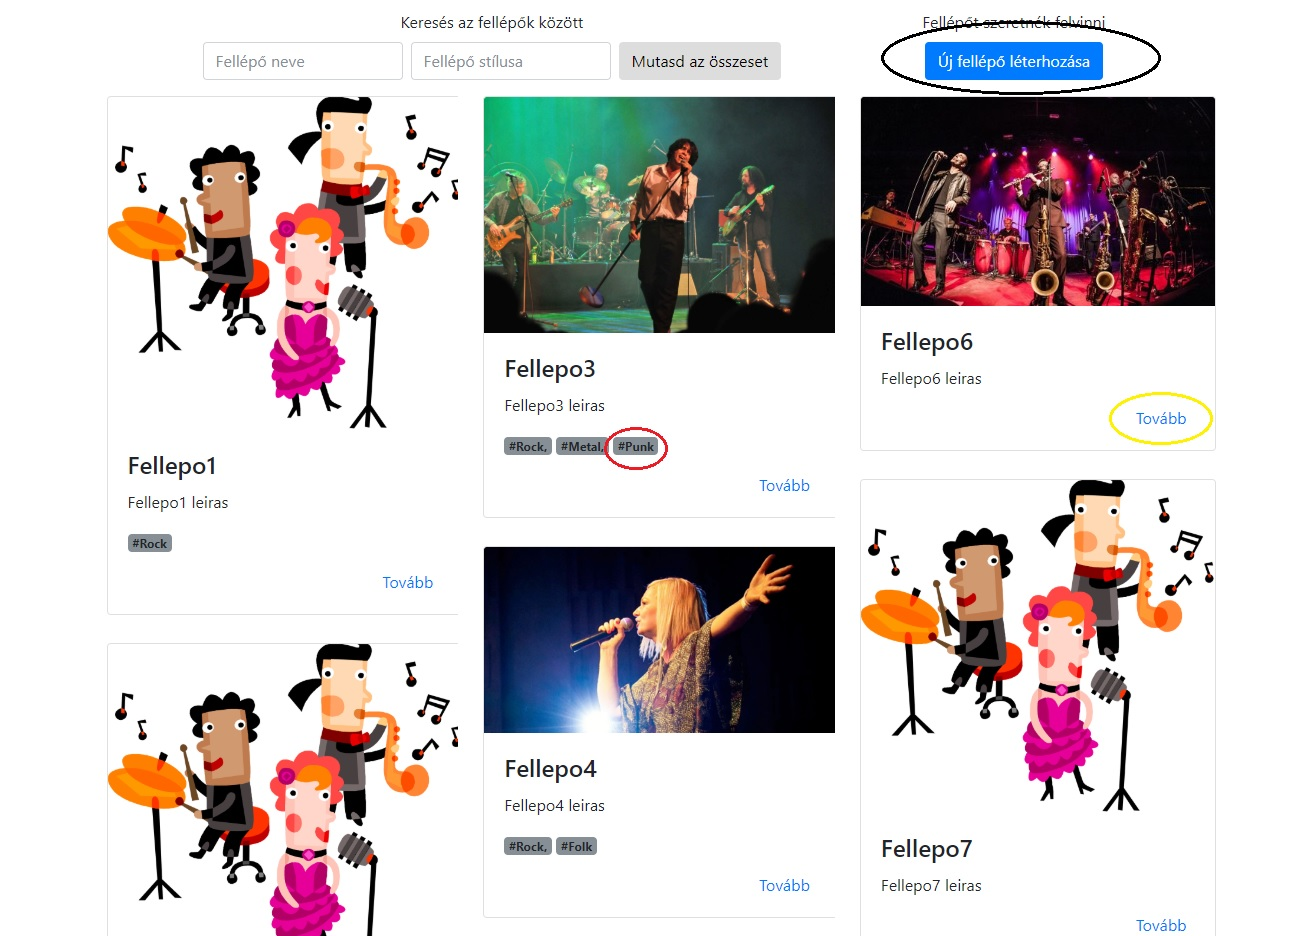
\includegraphics[scale=0.45]{kepek/artistList.jpg}
\caption{Fellépők listája}
\label{fig:artistList}
\end{figure}

Kezdjük a fellépők listázásával. A főmenüben a fellépőkre kattintással \aref{fig:artistList}. ábrán látható kép fogad bennünket. Amint látható, kilistázza a program az összes fellépőt, ami le van tárolva benne. Amelyikhez van kép is elmentve, ahhoz a képet is betölti, amelyikhez nincs, ahhoz pedig egy alapértelmezett képet rendel. A  két keresőmezőbe, ha beleírunk valamilyen szöveget, akkor leszűri azokra, amelyek tartalmazzák a beírt szövegrészletet értelemszerűen a fellépő nevénél a nevére, a stílusnál a stílusra szűr. Jobb felül a kék gomb (amit be is karikáztam), az csak akkor jelenik meg, ha a felhasználó bejelentkezik, és ahogy a felírata is mutatja új fellépő rögzítési helyéhez navigál. A stílusra kattintásra leszűri az olyan stílusuakra a halmazt, mint amire kattintottunk, ezt bordóval jelöltem. A továbbra kattintva a  fellépő részleteit ismerhetjük meg.

\begin{figure}[h!]
\centering
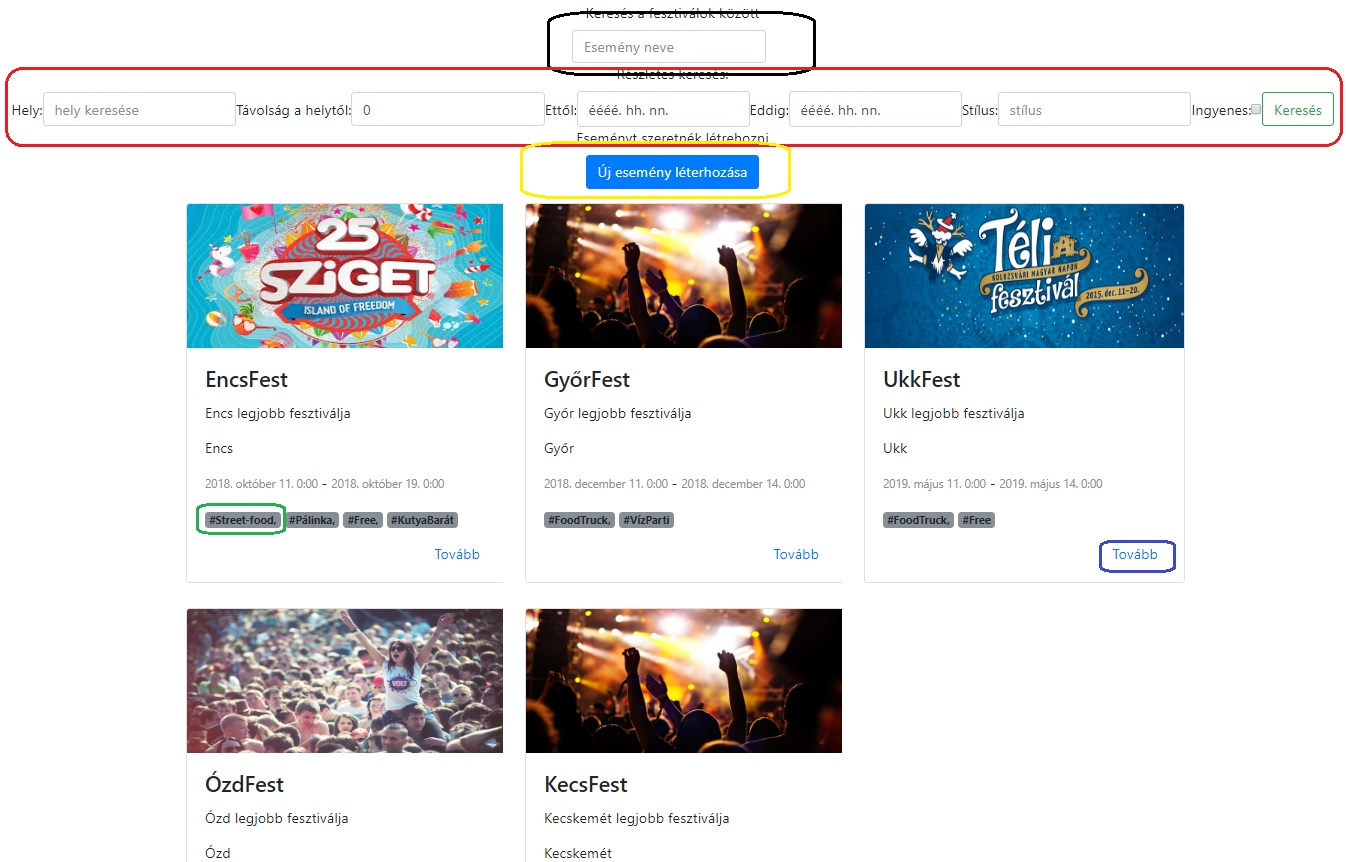
\includegraphics[scale=0.45]{kepek/festList.jpg}
\caption{Fesztiválok listája}
\label{fig:festList}
\end{figure}

Az első keresés az hasonló lesz, mint a fellépők listázásánál, viszont itt csak névre lehet a gombnélküli direktszűrő funkciót alkalmazni. A részletes keresés részt már kitárgyaltuk részletesen, ezt a funkciót a következő (piros blokkban) láthatjuk \aref{fig:festList}. ábrán. Sajnos nem nagyon értek a dízájnhoz, így kicsit összecsúsztak, de funkcióját tekintve működik. A többi dolog úgy működik, mint a fellépők listázásánál.

\begin{figure}[h!]
\centering
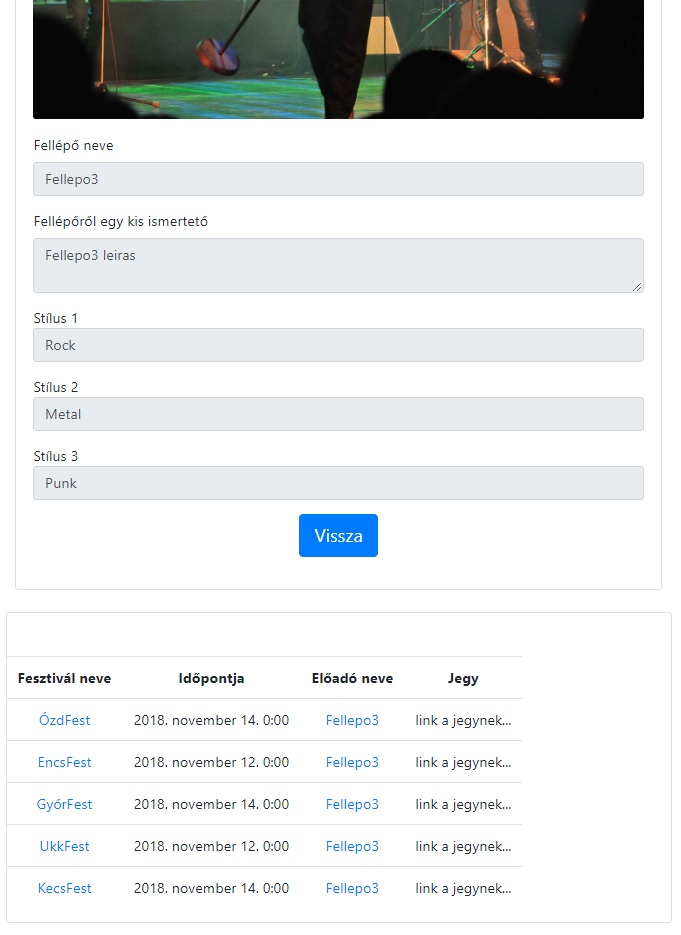
\includegraphics[scale=0.8]{kepek/artistDet.jpg}
\caption{Fellépők részletei}
\label{fig:artistDet}
\end{figure}

Fellépő részletei, amint \aref{fig:artistDet}. ábrán látható itt nem aktívak az input mezők, mert nem vagyunk belépve, ha belépünk akkor megjelenik egy szerkesztés gomb, és ha arra kattintunk akkor szerkeszthetjük az adatokat. Ezt meglehetett volna úgy is oldani, hogy nem input mezőbe vezetem ki a tulajdonságokat, hanem egy külön nézetet készítek a szerkesztésnek és a nem szerkeszthető résznek, és nem csak a szerkeszthetőségét tiltom le. Az alsó részen a fellépő koncert naptárát tekinthetjük meg.

\begin{figure}[h!]
\centering
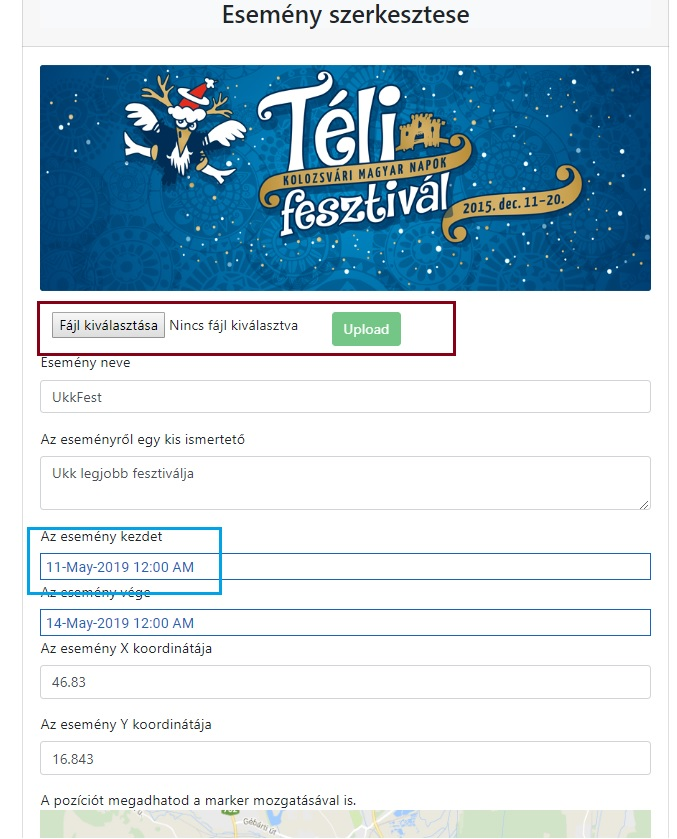
\includegraphics[scale=0.8]{kepek/eventDet.jpg}
\caption{Fesztiválok részletei}
\label{fig:event1Det}
\end{figure}

Esemény részletei, itt egy belépett felhasználó esetén láthatjuk aki rákattintott a szerkesztés gombra. A fesztivál képe alatt ilyenkor megjelenik a képfeltöltő blokk, ha kiválasztunk egy képet feltöltésre, akkor az upload gombra kattintva tölthetjük fel (\ref{fig:event1Det}. ábra). Az esemény kezdete és vége egy \textit{Date-Time-Picker} segítségével választható ki. Erre a későbbiekben mutatok is példát kinyitott állapotban. Az esemény koordinátáit lehet kézzel szerkeszteni vagy a térképen levő marker (fekete oválisban lévő piros tüske) segítségével megadható (\ref{fig:event2Det}. ábra). Ezt a markert csak szerkesztés módban lehet mozgatni. A lilával jelölt körben lévő X segítségével törölhetjük a stílusokat, illetve a narancssárga oválisban található feliratra kattintva újat hozhatunk létre. A mentéssel rögzíthetjük a változásokat. Új fesztivál felvitele esetén csak szimplán lementjük új fesztiválként. Ebből leszűrhetó az is, hogy ugyanezt az űrlapot töltjük be új felvitele esetén is. A törlésre kattintva törölhetjük a fesztivált az adatbázisból. 

\begin{figure}[h!]
\centering
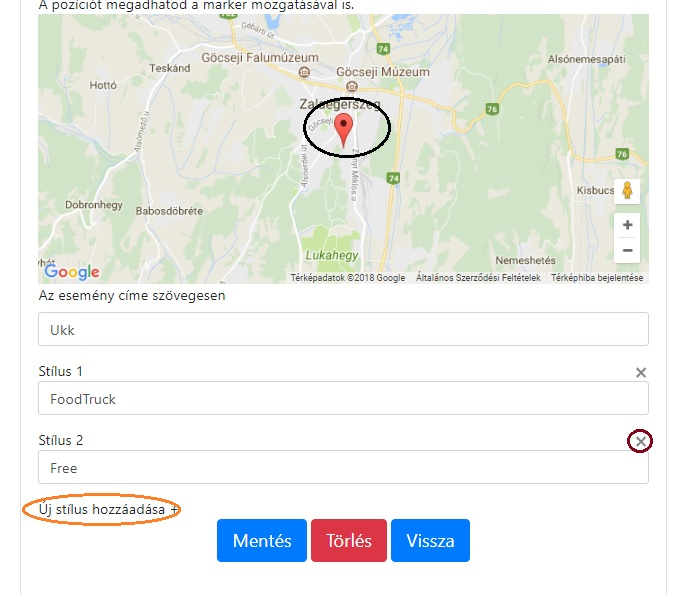
\includegraphics[scale=0.64]{kepek/eventDet2.jpg}
\caption{Fesztiválok részletei}
\label{fig:event2Det}
\end{figure}

A következő blokkban találjuk a fesztivál programját. Itt a fesztivál nevére kattintva elnavigálhatunk a fesztiválhoz, de ez az eset főleg a fellépőknél érdekes (\ref{fig:event3Det}. ábra). Az előadó nevére kattintva pedig az előadó részleteit tekinthetjük meg. Az utolsó részben pedig szállásokat ajánlunk a fesztiválozók számára, ezek a fesztiváltól maximum 5 km-re elhelyezkedő szállások lesznek. A tovább gombra kattintva elnavigáljuk a szállás weboldalára.

\begin{figure}[h!]
\centering
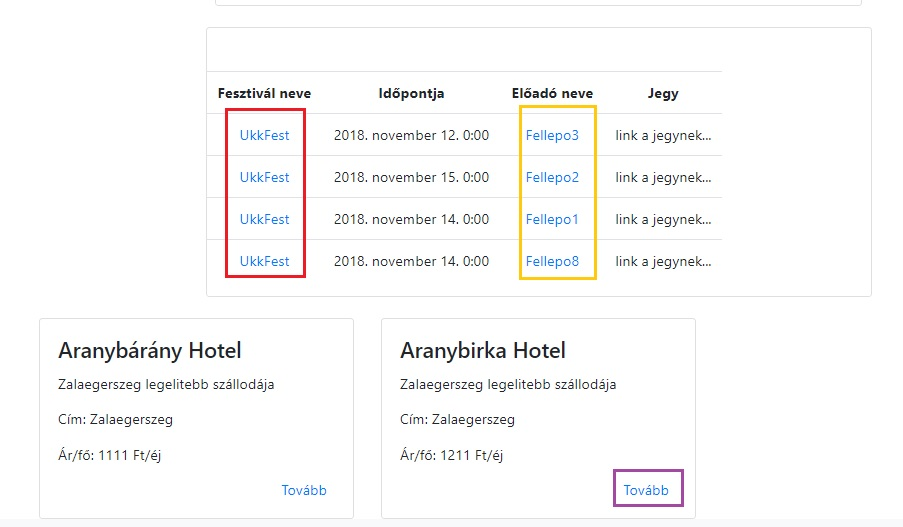
\includegraphics[scale=0.64]{kepek/festFoot.jpg}
\caption{Fesztiválok részletei}
\label{fig:event3Det}
\end{figure}

Az oldal fejlécét találjuk, itt találjuk a menüket, amik közül lehet választani. Az eseményekre kattintva jönnek be a fesztiválok listája, a fellépőkre kattintva a fellépők listája (\ref{fig:concert}. ábra). Az új szállás és az új koncert menü csak akkor jelenik meg a nav-bar-on, ha bejelentkezünk. A profile-ra írányít bennünket az oldal, ha sikerült belépnünk. A kilépéssel hagyhatjuk el az oldalt. Amíg nem lépünk be, addig az utolsó négy menü nem látszik, viszont van helyette bejelentkezés és regisztráció fül. A sárgával jelölt részen látható nyilak jelzik, hogy ez egy lenyilló lista. A listaelemek pedig a fesztiválok és a fellépők. A koncert időpontját itt is picker segítségével választhatjuk ki.

\begin{figure}[h!]
\centering
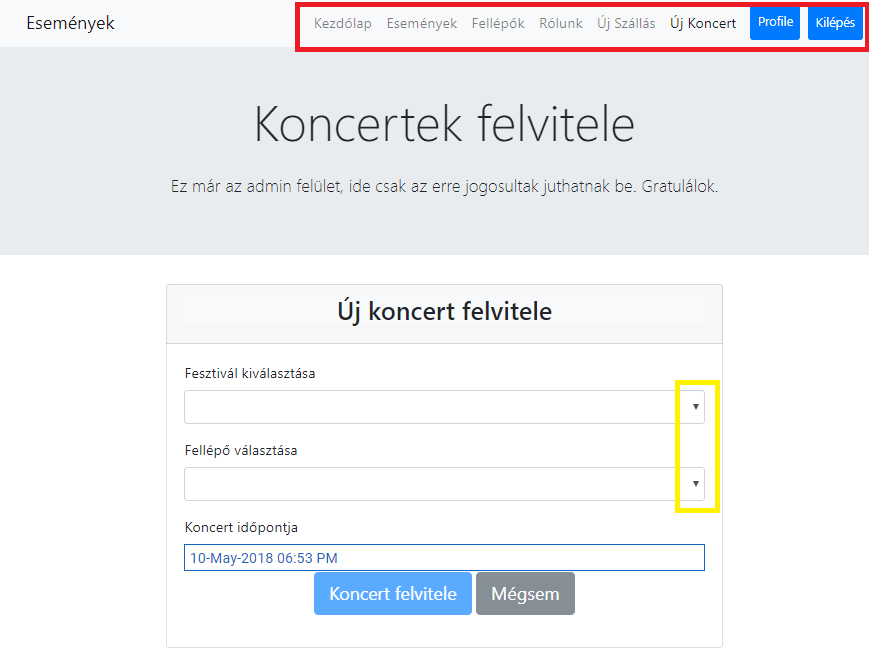
\includegraphics[scale=0.64]{kepek/concertUp.png}
\caption{Koncert rögzítése}
\label{fig:concert}
\end{figure}

A fesztivál listát láthatjuk kinyítva és a pickert (\ref{fig:concertOpen}. ábra). A fesztiválok listájában csak a még véget nem ért fesztiválok jelennek meg. A \textit{date-time-picker} segítségével pedig könnyedén kiválaszthatjuk a számunkra megfelelő dátumot.

\begin{figure}[h!]
\centering
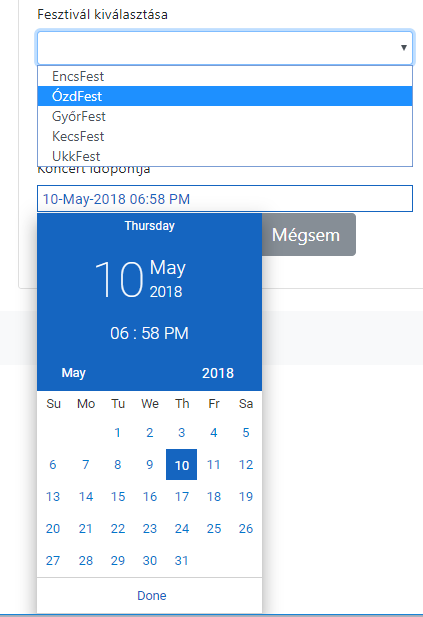
\includegraphics[scale=0.64]{kepek/concertUpOpen.png}
\caption{Koncert rögzítése}
\label{fig:concertOpen}
\end{figure}

\Chapter{Telepítés, tesztelés}

% TODO: Az alkalmazás üzembehelyezését, konfigurációját részletesen bemutatni!

% TODO: Példa néhány felhasználói tesztre. Le lehet írni, hogy mi az amit közben korrigálni kellett. A javítás módját is le lehet írni.

% TODO: Frontend teszteléséhez használható eszközök bemutatása és néhány konkrét példa a tesztekre.

% TODO: Java egységtesztek bemutatása. Például kereséshez, szűréshez, regisztrációhoz.
\section{Telepítés}

Mindkét keretrendszer független az operációs rendszerektől, tehát minden népszerű operációs rendszert használó számítógépen el tudjuk indítani az alkalmazásokat.

\subsection{Spring}

A Spring Boot 1.5.8.RELEASE kiadást használtam, ez a Java 7-es verzióját igényli - a 8 vagy újabb ajánlott - a fordításhoz. Tehát érdemes telepíteni a lehető legújabb Java-t, mind a JRE-t mind a JDK-t.

Maven segítségével töltjük le azokat a jar fájlokat amelyektől függ az alkalmazásunk. A 3.5.0 verzió volt akkor a legújabb verzió és általam használt verzió is ez. A Maven 3.5.0 szintén igényli a Java hetedik verzióját vagy újabb kiadásait. A projekt pom.xml fájljában definiált csomagok az alkalmazás függőségei, ezeket a fordítás előtt le fogja tölteni, ha nem találja meg őket az erre a célra lefoglalt mappában. Ezeknek a csomagoknak vannak további függőségeik, azokat is feloldja a Maven, amíg a függőségi fán hiányzó levelet talál, addig folytatja ezt az eljárást. Így levesz minden terhet a vállunkról.

\subsection{Angular}

[31] A front-end részhez először telepíteni kell egy Node.js-t. Az akkor elérhető legfrissebb verziót, amely a 9.10.1 volt. Ez a keretrendszer weboldaláról(nodejs.org) letölthető. Erre azért volt szükségünk, mert ebben található egy npm nevű modul. Az npm vagy Node Package Manager, mint a neve is mutatja csomagok telepítésére és karbantartására való.

Egy csomagot kétféleképpen lehet installálni az egyik a helyi telepítés és a globális telepítés. Globálisan olyan csomagokat szokás telepíteni amiket többnyire terminálból akarunk futtatni.
Mi az Angular CLI 1.7.0-t globálisan telepítettük npm segítségével, hiszen parancssorból szeretnénk indítani majd a kiszolgálást.

A következő paranccsal érhetjük ezt el, hogy a legfrissebb verziót telepítse: \texttt{npm install -g @angular/cli}
Elvileg visszafelé kompatibilis a rendszer, tehát ha a legújabb globális verzió van fent a gépen akkor a régebbi vagy azonos verziószámú projektet képes lesz futtatni. Én Angular 5.2.0-ás verziószámú projektet futtattam benne, és minden gond nélkül elindult.
Minden projekthez tartozik egy \texttt{package.json}, úgy mint a Maven-nél a \texttt{pom.xml}, ez tárolja a projekt függőségeit. Ezeket le kell tölteni, ha van olyan amelyik nincs telepítve, én ezt már lokálisan tettem meg. Terminál segítségével ezt úgy tehetjük meg, hogy benavigálunk a projekt mappájába és futtatjuk az \texttt{npm install} parancsot, jelentősebb időbe telik mire letölt mindent amire szükség lesz a projekt futtatásához. Majd ezután, ha minden rendben ment, akkor az \texttt{ng serve} parancsra elkezd futni a program. A terminálra kiírja, hogy melyik porton indult el, ez a \texttt{localhost:4200} gyári beállításon. Ha a back-end oldali alkalmazás is fut a \texttt{localhost:8080}-as porton, akkor már az adatok is vizualizálódnak.

\section{Tesztelés}

\subsection{Felhasználói felület tesztelése}
A felhasználói felületet funkcionális tesztekkel manuálisan tudtam tesztelni, hogy minden úgy működik-e, ahogy azt a rendszertől elvártam. A tesztelés másik módja az volt, hogy JSON pipe segítségével megjelenítettem az adatokat a felületen, és így valós időben tudtam követni az interakcióim hatására bekövetkező változásokat. Van lehetőség a funkcionális tesztek automatizálására a front-end oldalon, de időmből nem futotta ennek elsajátítására.

\subsection{Back-end tesztelése}

A Spring-nél szokás használni a tesztelés által irányított fejlesztést(TDD), ez azt jelenti hogy először megírjuk a teszteket és utána a kódot hozzá. Minden modul akkor áll készen, ha definiált tesztek sikeresen lefutottak. Majd jöhet a következő modul, viszont azt már úgy kell elkészítenünk, hogy a saját tesztjei is lefussanak, illetve a régebben elkészített modulok tesztjei is sikeresek maradjanak. Én nem így készítettem el a modult, csak már a kész modulokat teszteltem.

Először a back-enddel készültem el, és nem volt felhasználói felületem(UI) aminek segítségével az egyes kéréseket szimulálhattam volna, így Postman segítségével küldtem be a minta kéréseimet és ezáltal teszteltem fejlesztési időben. 

Egység teszt, ezzel egyetlen egy metódus működését tesztelhetjük, csak a  legelemibb megoldásokat tesztelhetjük vele.

Az egység tesztek után az integrációs teszteket szokták elvégezni, azt vizsgálja, hogy a modulok jól tudnak-e együttműködni.

Stresszteszteket JMeter segítségével készítettem. A stressztesztek arra használatosak, hogy kiderítsük mekkora aktivitásnak tehetjük ki az alkalmazást.
\Chapter{Összegzés}


\begin{thebibliography}{x}
\addcontentsline{toc}{chapter}{\bibname}

% TODO: Angular-ral, JavaScript-el kapcsolatos irodalmak.

% TODO: Java alapkönyv, keretrendszerekről néhány, Spring

% TODO: A fesztiválkereső alkalmazások webcímei

[1]\url{ http://mfdesign.hu/cikkek/reszponziv_design } %idézet

[2]\url{ https://martinfowler.com/articles/injection.html }

[3]\url{ https://spring.io/ }

[4]\url{ https://angular.io/ }

[5]\url{ https://github.com/minutuslausus }

[6]\url{ http://sanfranciscoboljottem.com/ }

[7]\url{ https://docs.oracle.com/javaee/6/tutorial/doc/docinfo.html }

[8]\url{ https://www.ibm.com/developerworks/webservices/library/ws-restful/ }

[9]\url{ https://stackoverflow.com/questions/10604298/spring-component-versus-bean }

[10]\url{ http://nyelvek.inf.elte.hu/leirasok/TypeScript/index.php?chapter=1 }

[11] Dr. Kovács László: Adatbázis Rendszerek I.

[12] Dr. Kovács László, Dr. Pance Miklós: Adatmodellezés és adatkezelési technikák (2011)

[13]\url{ http://www.memooc.hu/ }

[14] Antal Margit: Java alapú webtechnológiák, Scientia Kiadó, Kolozsvár, 2009.

[15]\url{ https://www.portfolio.hu/gazdasag/ezek-a-fesztivalok-atrendezik-magyarorszag-turisztikai-terkepet.233802.html } %cikk alapján következtetés

[16]\url{ https://turizmus.com/desztinaciok/duborog-a-fesztivalturizmus-1130113 } %cikk alapján következtetés

[17]\url{ https://nodejs.org/en/ }

[18] Ficsor Lajos, Dr. Kovács László, Krizsán Zoltán, Dr. Kusper Gábor: Szoftvertesztelés

[21]\url{ http://www.fesztivalszovetseg.hu/ } %idézet

[22] Dr. Millisits Endre HASHTAGEK ÉS VÉDJEGYOLTALOM

[23] \url{ https://docs.spring.io/spring-boot/docs/current/reference/html/getting-started-system-requirements.html }

[31] \url{ http://nodehun.blogspot.hu/2015/05/mi-az-az-npm.html } %idézet

\end{thebibliography}


\Chapter{CD-melléklet tartalma}

A dolgozatomhoz mellékeltem egy CD-t, amely az alábbiakat tartalmazza.

\begin{itemize}
\item \texttt{dolgozat.pdf}: A szakdolgozat PDF formátumban.
\item \texttt{dolgozat} jegyzék: A szakdolgozat \LaTeX\ forrása.
\item \texttt{festapp} jegyzék: A fesztiválszervező alkalmazás forráskódja.
\end{itemize}

\bigskip

\noindent A dolgozathoz készített alkalmazás aktuális forráskódja elérhető GitHub-on az alábbi címen.
\begin{itemize}
\item \url{https://github.com/martinb91/festapp}
\end{itemize}


\end{document}
